\section{Architettura}

Per l'architettura dell'applicativo da sviluppare si è deciso di utilizzare
\textit{Model-View-ViewModel}, derivato da \textit{Model-View-Controller}.

\subsection{Viste}
% TODO: Viste non nel senso del pattern
Per garantire l'uniformità e la riusabilità di tutti i componenti delle varie
viste si è deciso di utilizzare per tutti la stessa struttura.

\subsubsection{Caratterizzazione di una vista}
Una vista è caratterizzata da:
\begin{itemize}
  \item Tipo di grafico (scatterplot, parallel coordinates, ecc...).
  \item Impostazioni di rendering.
  \item Associazione degli assi alle dimensioni del grafico.
\end{itemize}

\subsubsection{Logica di Rendering}
\begin{itemize}
  \item Renderer: componente che si occupa di adattare (Adapter pattern) il
    meccanismo di rendering delle varie librerie alla nostra architettura
    specifica, in particolare esso opera sui nostri oggetti di dominio come il
    dataset$^{G}$ già preparato per il render$^{G}$ (ad esempio mappati come punti 2
    dimensionali nello scatterplot$^{G}$) e le sue impostazioni specifiche di
    rendering$^{G}$ (ad esempio lunghezza degli assi x ed y nello scatterplot$^{G}$)
    traducendoli in un formato comprensibile dalla libreria di supporto.
  \item Mapper: componente che si occupa di trasformare il dataset$^{G}$ generale nel
    dataset$^{G}$ preparato per il render$^{G}$.
\end{itemize}

\begin{figure}[h!]
  \centering
  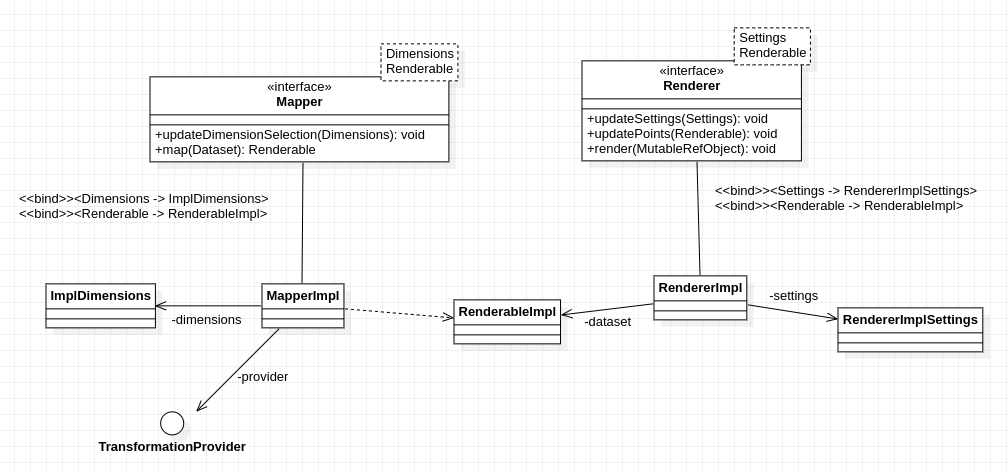
\includegraphics[scale=0.60]{../../assets/classi_uml/modelvista.png}
  \caption{Esempio di implementazione di una vista di tipo \texttt{Impl}.}
\end{figure}
\newpage
\subsubsection{Interazione con l'utente}
L'utente deve poter interagire con l'applicazione per poter modificare
preferenze del grafico specifico, quindi si utilizza mvvm per modellare questa
interazione. Il componente verrà generato utilizzando la libreria \texttt{MobX}.

\begin{figure}[h!]
  \centering
  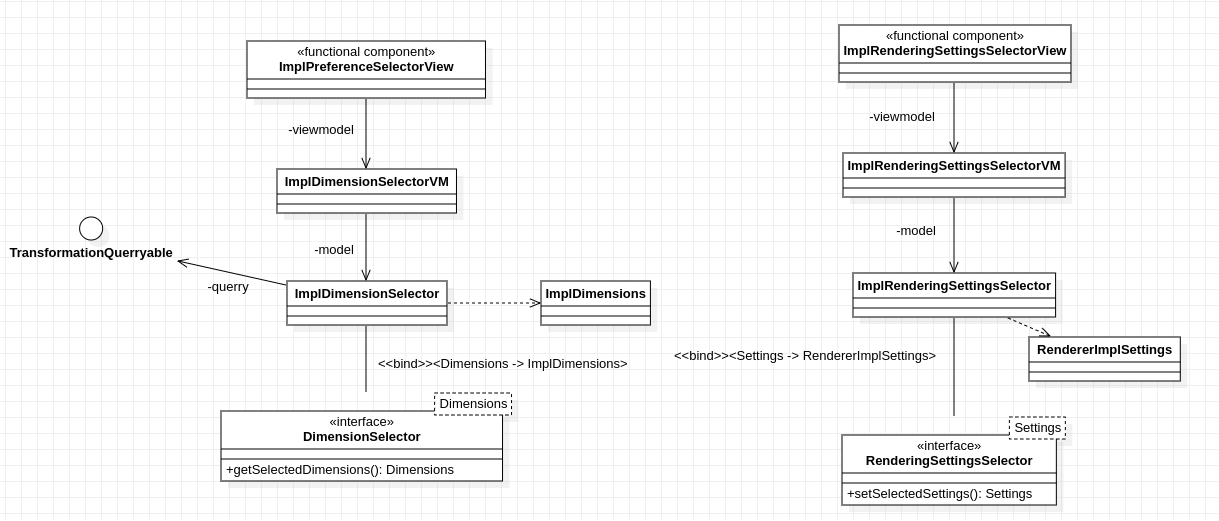
\includegraphics[scale=0.55]{../../assets/classi_uml/modelinterazione.png}
  \caption{Esempio di implementazione dell'interazione di tipo \texttt{Impl}.}
\end{figure}

\subsubsection{Composizione}
Per creare una vista completa sì utilizzerà un componente generico in modo da
favorire la composizione e creazione di nuove tipologie di vista, senza dover
interagire con il codice che si occupa di manipolare il flusso dei dati che vista
la nostra architettura risulta essere standard, senza perdere di flessibilità.

\begin{figure}[h!]
  \centering
  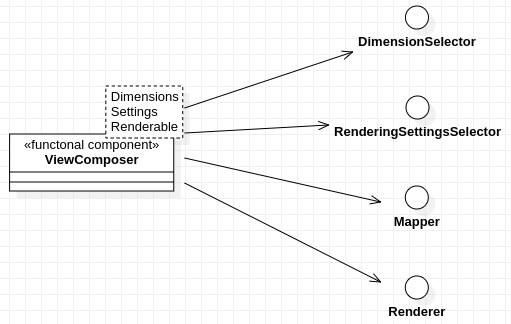
\includegraphics[scale=0.55]{../../assets/classi_uml/comdelcomposer.png}
  \caption{Dimostrazione di composizione generica}
\end{figure}

Questo permette di riutilizzare al massimo tutta la logica comune (grazie al fatto
che le varie componenti implementano tutte una interfaccia) non si è deciso di usare
il pattern \texttt{TemplateMethod} in quanto i componenti di react devono essere
funzioni (I class components sono deprecati).

Risulta estremamente flessibile anche nel caso si voglia cambiare anche un solo
componente ad esempio fornire un dimension selector sullo ScatterPlot.

\begin{figure}[h!]
  \centering
  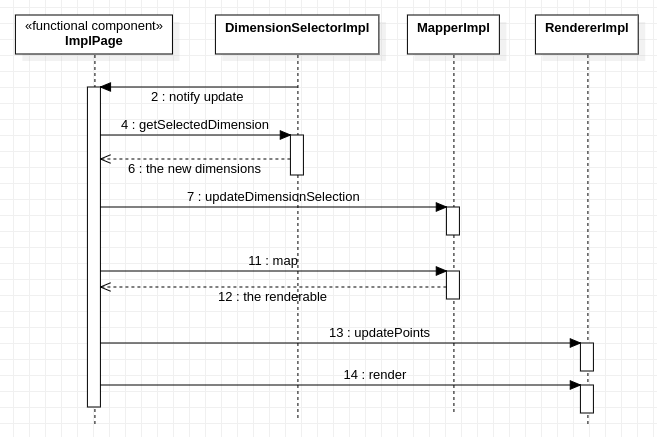
\includegraphics[scale=0.55]{../../assets/classi_uml/interazione_gw.png}
  \caption{Dimostrazione dell'orchestrazione dell' aggiornamento delle
    dimensioni da parte di generic view, ovviamente per semplcità sono riportate
    le solo i modelli e non anche le loro view e viewmodel.}
\end{figure}

\subsection{Stato dell' applicazione}
L'applicazione ha uno stato con cui tutte le viste interagiscono.
\begin{itemize}
  \item Viste create dall'utente in precedenza.
  \item Trasformazioni sui dati disponibili.
  \item Dataset$^{G}$.
\end{itemize}

\subsubsection{Trasformazioni}
Il transformer è la classe che mantiene traccia di tutte le trasformazioni (cioè
funzioni che trasformano un campo di una entry del dataset in qualcosa che il
renderer è in grado di disegnare). \\
Esso espone 2 interfacce così da segregarne l'uso, una è destinata alla ricerca di
trasformazioni (TransformationQuerryable) e l'altra al riferimento delle stesse tramite
signature (TransformationProvider). \\
\begin{figure}[H]
  \centering
  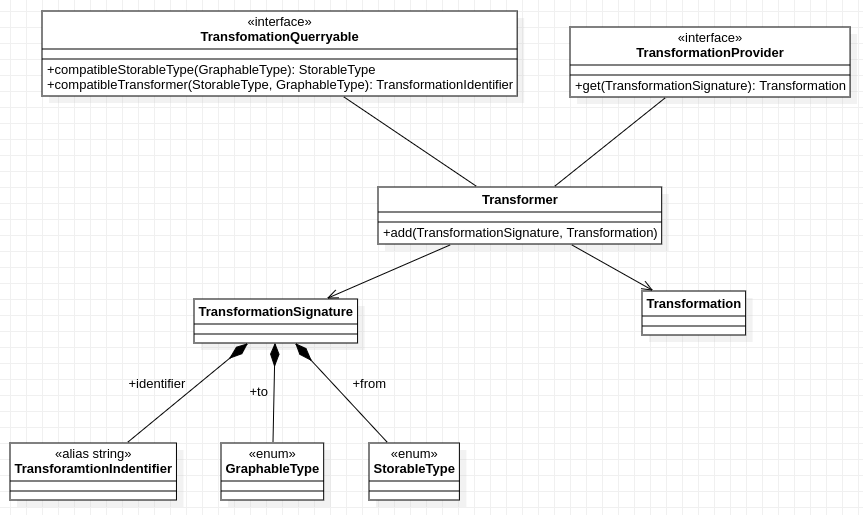
\includegraphics[scale=0.65]{../../assets/classi_uml/modeltransfomer.png}
\end{figure}
Questo modella il \texttt{Repository} che si occupa di eseguire query
basate su constraints (e.s. Trasformazioni che possono trasformare un intero
in un colore) quindi \\ \texttt{TransformationQuerryable} o in base all'id
\texttt{TransformationProvider}, non sono state implementante altre operazioni
tipiche \texttt{CRUD} in quanto non risultano essere necessarie e avrebbero
solo aumentato la complessità del codice senza un motivo valido.

Inoltre Transformer è anche un singleton.

\subsubsection{Dataset}
Il dataset$^{G}$ raggruppa i dati caricati dall'utente in una collezione di
\texttt{DatasetEntry} che non sono altro che una collezione di coppie nome del
campo e valore (uno storable type). \\
\begin{figure}[H]
  \centering
  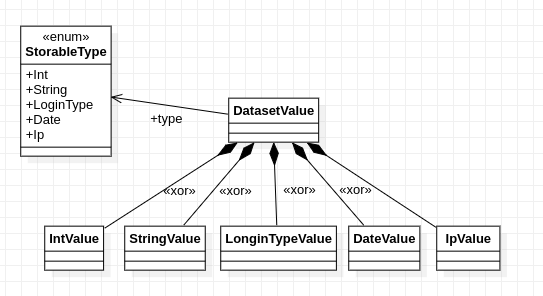
\includegraphics[scale=0.65]{../../assets/classi_uml/datasetentrypng.png}
\end{figure}
Tramite la modellazione tramite sumtype e l'utilizzo di typelevel function
possiamo operare su un dataset eterogeneo mantenedo comunque typesafety.
\begin{verbatim}
  export type StorableTypeToRepr<T extends StorableType>
    = T extends StorableType.Int ? Int
      : T extends StorableType.String ? string
        : T extends StorableType.Date ? Date
          : T extends StorableType.Ip ? string
            : LoginType;
\end{verbatim}
Esempio di typelevel function che trasforma una istanza dell'enum
\texttt{StorableType} nel tipo che rappresenta.
\\

\noindent
Il dataset non è altro che un insieme di \texttt{DatasetEntry} che rappresentano
una riga del dataset in un qualsiasi momento dell' elaborazione, una entry è un
insieme di field accompagnati dal loro tipo così da poter mostrare all'utente
solo opzioni sensate di rendering all'utente, il dataset espone la sua signature
cioè i suoi campi e loro tipo così da permettere introspezione su di esso.\\

\begin{figure}[h!]
  \centering
  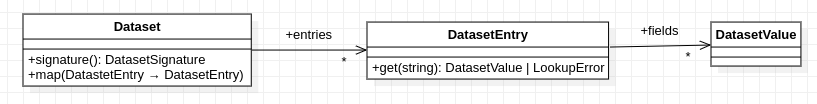
\includegraphics[scale=0.55]{../../assets/classi_uml/dataset.png}
  \caption{Dataset e DatasetEntry}
\end{figure}

\noindent
Per mettere l'estrazione di dati derivati il dataset espone un metodo di map,
simile a quello presente sulle varie collezioni standard inJavaScript/Typescript,
è possibile attivare o disattivare il check della signature del dataset.

\paragraph{Parsing del Dataset:}
Per rendere l'applicazione il più agnostica possibile al formato del dataset
(questo può tornare utile in caso si trovino altri dataset interessanti nella
fase esplorativa ed è praticamente gratis da implementare) si è deciso di
nascondere l'operazione dietro una interfaccia \texttt{DatasetParser}, questo
tipo di architettura risulterà anche molto flessibile in quanto potrà anche
essere parallelizzata facilmente in formati in cui il contesto è la singola
linea tipo \texttt{CSV} aggregandone più diversi.
\begin{figure}[h!]
  \centering
  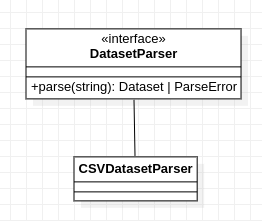
\includegraphics[scale=0.55]{../../assets/classi_uml/datasetparser.png}
  \caption{DatasetParser}
\end{figure}

\paragraph{Caricamento del Dataset:}
Sempre seguendo la stessa filosofia del parsing anche il caricamento del dataset
è implementato tramite l'interfaccia \texttt{DatasetProvider} questa poi allo stato
attuale viene implementata sia da \texttt{HTTPDatasetProvider} (ovviamente non ci
sono problemi per il supporto di HTTPS) che da \texttt{DragAndDropDatasetProvider}, in
futuro si potrebbe anche creare un Dataset Provider anche per lo storage locale del
Browser. Tutte queste ovviamente utilizzano la dependency injection per rimanere
agnostici al formato del dataset ricevendo una istanza di \texttt{DatasetParser}
alla costruzione.
\begin{figure}[h!]
  \centering
  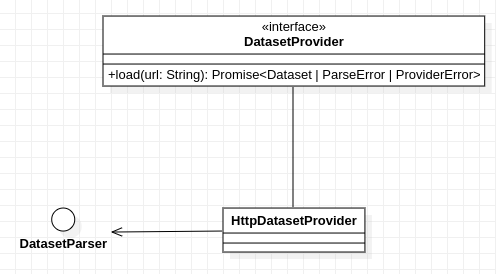
\includegraphics[scale=0.55]{../../assets/classi_uml/datasetprovider.png}
  \caption{DatasetProvider}
\end{figure}
Ovviamente le operazioni sono trattate come asincrone in modo da poi non
bloccare il rendering della user interface.

\subsubsection{Viste utilizzabili dall'utente}
Le viste sono il raggruppamento delle preferenze del grafico e delle dimensioni
scelte dall'utente durante la fase esplorativa. Le viste sono salvate all'interno
di \texttt{FullView} che raggruppa più viste differenti come quella dello
ScatterPlot e Sankey.
\begin{figure}[h!]
  \centering
  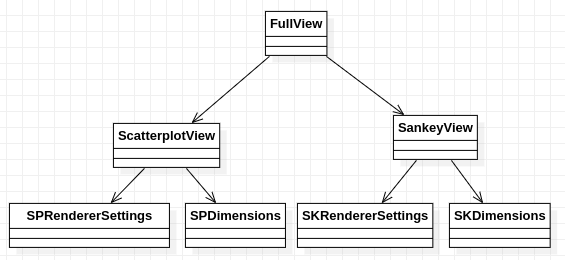
\includegraphics[scale=0.55]{../../assets/classi_uml/vister.png}
  \caption{Viste}
\end{figure}

\paragraph{Salvataggio e caricamento viste}
I tipi delle varie viste (Dimensioni e Preferenze) sono agglomerati all'interno
del tipo somma \texttt{View} così da poter essere facilmente identificate
discriminando il campo \texttt{type}, queste vengono serializzate e
deserializzare dal formato \texttt{JSON} dalle classi \texttt{ViewSerializer} e
\texttt{ViewDeserializer}

\begin{figure}[h!]
  \centering
  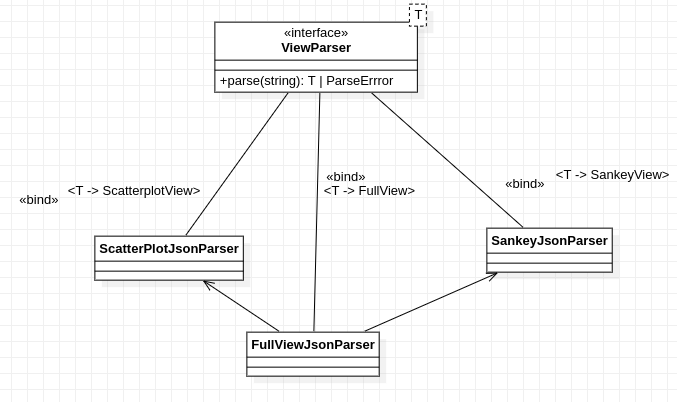
\includegraphics[scale=0.55]{../../assets/classi_uml/viewparser.png}
  \caption{ViewParser}
\end{figure}

\begin{figure}[h!]
  \centering
  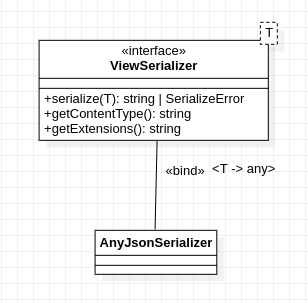
\includegraphics[scale=0.55]{../../assets/classi_uml/viewserializer.png}
  \caption{ViewSerializer}
\end{figure}

Inoltre il \texttt{ViewSerializer} espone metodi per permettere alla logica di salvataggio
di comprendere come costruire il file in cui salvare l'istanza serializzata.

\subsection{Componenti}
Al cuore di qualsiasi applicativo scritto con la libreria React per tutte le
funzionalità implementate dal punto di vista di modello (ad esempio: Caricamento e Parsing
del dataset, caricamento e parsing delle viste create da utente) sono stati creati degli
appositi functional components sempre sfruttando la dependency injection, alcuni esempi sono:
\begin{itemize}
  \item \texttt{LoadDatasetView}
  \item \texttt{ViewsDownloaderView}
  \item \texttt{ViewsLoaderView}
\end{itemize}

\begin{figure}[h!]
  \centering
  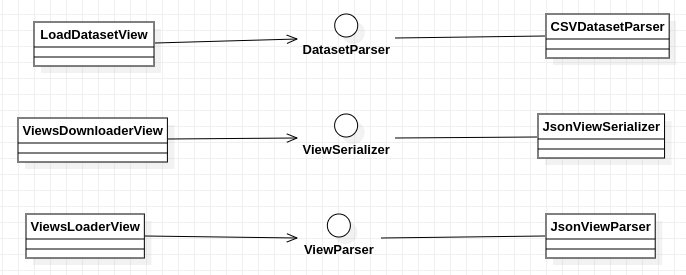
\includegraphics[scale=0.55]{../../assets/classi_uml/components.png}
  \caption{Alcuni dei componenti}
\end{figure}

Questo come si può intuire grazie alla dependency injection oltre a rendere
facile il testing permette anche di cambiare il comportamento di alcuni componenti
senza cambiare nulla (es: Dataset in formato JSON e Views in formato CSV).

\subsection{Routing}
La possibilità di poter cambiare vista selezionata è parte integrante dell'esperienza
di utilizzo dell' applicativo, il routing è gestito tramite la libreria
\texttt{react-router} e con la creazione delle varie route che permettono all'utente di
spostarsi tra le varie pagine dell'applicazione mantenendo uno stato valido

\subsection{Composizione elementi di UI}
Una visione ad alto livello della composizione dei vari elementi di UI, si nota in
particolare che i vari \texttt{Renderer} non ne fanno parte in quanto non sono
loro stessi ad essere parti della vista in quanto essi sfruttano un \texttt{div}
facente parte del \texttt{DOM HTML} sul quale posizionare il render
fatto tramite \texttt{WebGL}.

\begin{figure}[h!]
  \centering
  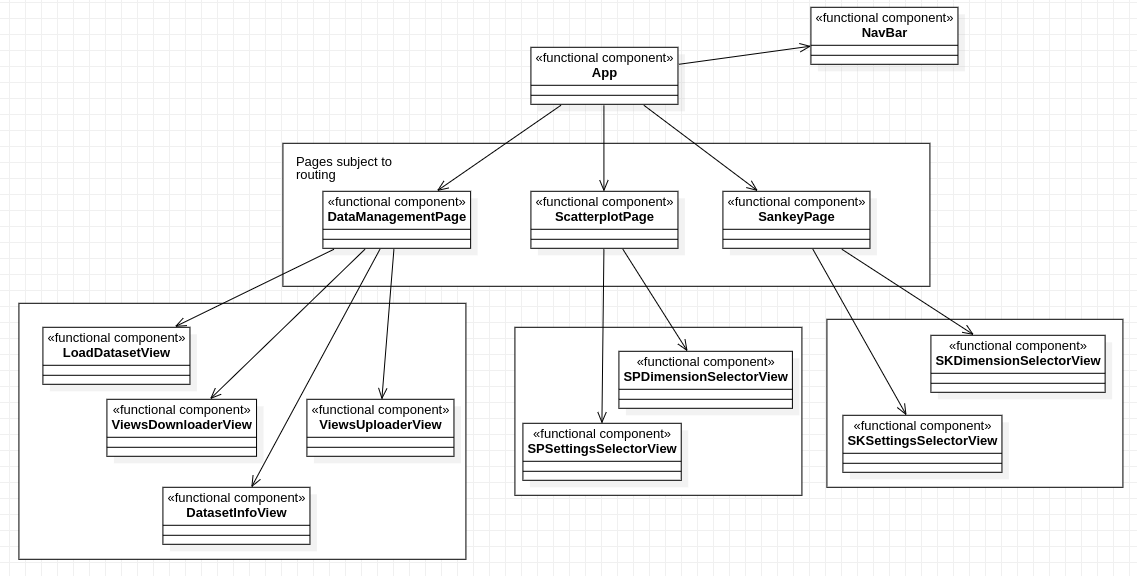
\includegraphics[scale=0.55]{../../assets/classi_uml/vistaglobale.png}
  \caption{Alcuni dei componenti}
\end{figure}

Sono presenti solo i componenti esportati dai vari file \texttt{.tsx} in quanto i vari
sotto componenti più piccoli non sono interessanti ai fini architetturali e non li si vuole
esporre in quanto potrebbero creare dipendenze non necessarie.

\subsubsection{Proprietà dello stato globale}
Lo stato dell'applicazione è gestito tramite gli hook di \texttt{React} per questo è importante
evidenziare che componenti possiedono, modificano e leggono esso per comprendere la dipendenze
e quali componenti effettivamente subiscono un render quando c'è un aggiornamento.

I componenti dello stato mutabile sono posseduti dal componente \texttt{App} che poi distribuisce
i getter e i setter generati dallo \texttt{stateHook} tramite i props dei vari componenti.

Perché non si è utilizzato \texttt{redux} o similari per la gestione dello stato? Lo stato
non è sufficiente complesso per giustificare l'introduzione di tale complessità extra inoltre
rende meno chiare le dipendenze (che ora sono facilmente visibili tramite la struttura dei
vari props) e inoltre non sarebbe typesafe cosa che invece all'interno dell' applicazione
ci si è impegnati a mantenere.

% \subsection{Diagrammi dei package}
% \subsection{Diagrammi delle classi}

% \subsubsection{View}

% \begin{figure}[h!]
    % \centering
    % 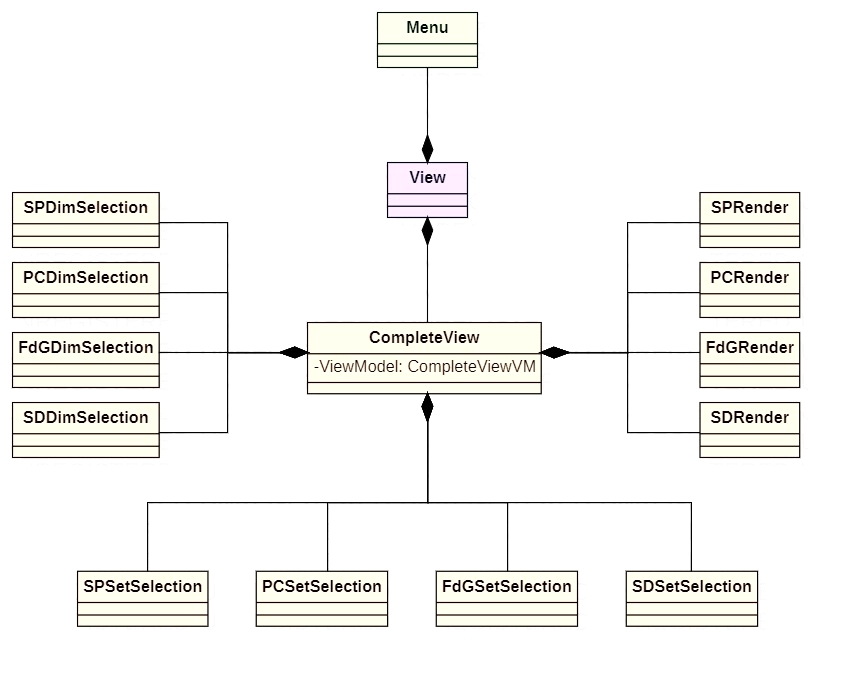
\includegraphics[scale=0.75]{../../assets/classi_uml/View.jpg}
    % \caption{Diagramma delle classi - View}
% \end{figure}
% \newpage
% \subsubsection{Model}

% \begin{figure}[h!]
    % \centering
    % 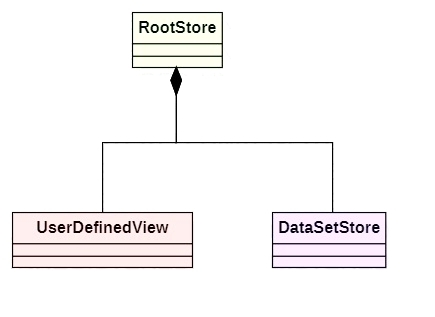
\includegraphics[scale=0.75]{../../assets/classi_uml/Model.jpg}
    % \caption{Diagramma delle classi - Model}
% \end{figure}

% \subsection{Diagrammi di sequenza}
